\subsection*{Задание 1.2}

\underline{Условие:}  Все потоки случайных событий считать пуассоновскими. Если все операторы заняты, звонок теряется. Построить график изменения доли отказов при замене каналов обслуживания местами в очереди (начиная с числа операторов, соответствующего 1\% отказов в системе без очереди). Построить график, иллюстрирующий коэффициент загрузки операторов. Построить график математического ожидания длины очереди. Построить график, иллюстрирующий коэффициент занятости мест в очереди. Построить график математического ожидания времени пребывания клиентов в очереди. 
\\

Решение:
Из задачи 1.1 известно, что при количестве операторов  N = 16 вероятность отказа системы составляет 0.6 \%. Для расчета вероятности, при которой операторы не будут заняты.
Тогда вероятность того, что операторы не заняты вычисляется по формуле:

\begin{equation}
    P_{0} = \frac{1}{\sum_{i=0}^{N} \frac{\lambda^i}{i! \mu^i}+\frac{\lambda^N}{N! \mu^N} \sum_{k=1}^{M}{(\frac{\lambda}{N \mu})^k}}
\end{equation}
, где M - количество мест в очереди.

Для расчета вероятности отказа системы можно воспользоваться формулой:

\begin{equation}
    P_{den} = \frac{\lambda^N}{N! \mu^N} (\frac{\lambda}{N \mu})^M P_0
\end{equation}

Расчет среднего количества занятых операторов ведется по формуле:

\begin{equation}
    \overline{N} = \sum_{i=0}^{N} i P_i + \sum_{k=1}^{M} N P_k
    \label{Naver}
\end{equation}

Матожидание длины очереди ведется по формуле:
\begin{equation}
    \overline{Q} = \sum_{k=1}^{M} k P_k
    \label{}
\end{equation}, 
где $\overline{Q}$ - матожидание длины очереди. Коэффицент занятости мест в очереди вычисляется по формуле:
$k = \frac{\overline{Q}}{Q}$, где k - коэффициент занятости мест в очереди.

Среднее время ожидания в очереди вычисляется по формуле: \\$\Delta \overline{t} =  \frac{\overline{Q}}{\lambda}$.  


\begin{figure}[H]
	\begin{center}
        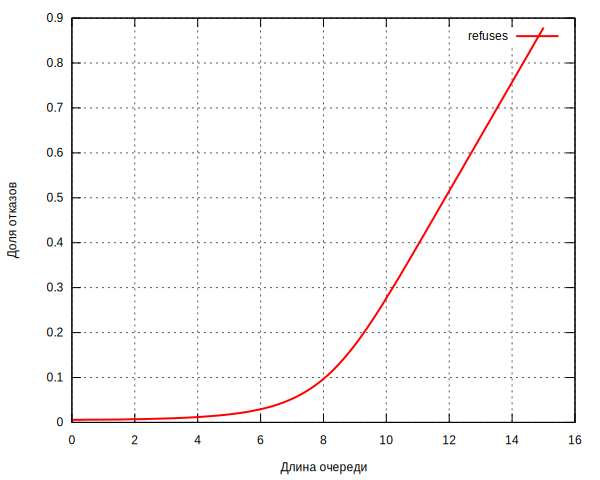
\includegraphics{/z1.2/qref.pdf}
        \caption{Зависимость вероятности отказа системы от мест в очереди}
	\end{center}
\end{figure}

\begin{figure}[H]
	\begin{center}
        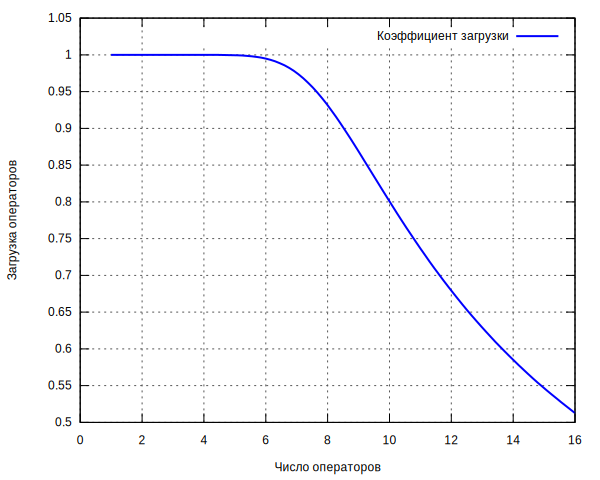
\includegraphics{/z1.2/kcpref.pdf}
        \caption{Зависимость коэффициента загрузки операторов от их общего количества}
	\end{center}
\end{figure}

\begin{figure}[H]
	\begin{center}
        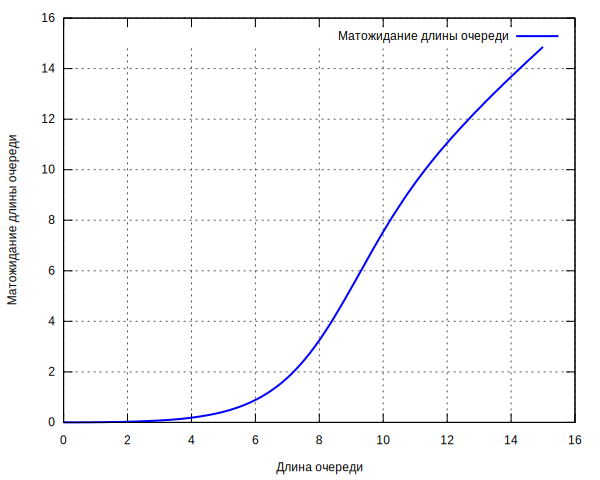
\includegraphics{/z1.2/matozh.pdf}
        \caption{Зависимость математического ожидания длины очереди от мест в очереди}
	\end{center}
\end{figure}

\begin{figure}[H]
	\begin{center}
        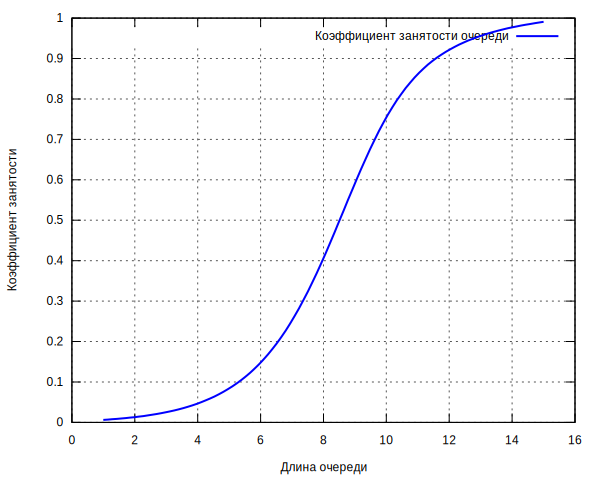
\includegraphics{/z1.2/queucoeff.pdf}
        \caption{Зависимость коэффициента занятости мест в очереди от длины очереди}
	\end{center}
\end{figure}

\begin{figure}[H]
	\begin{center}
        \includegraphics{/z1.2/qwtime.pdf}
        \caption{Зависимость математического ожидания времени ожидания в очереди от мест в очереди}
	\end{center}
\end{figure}